\documentclass[]{article}
\usepackage{lmodern}
\usepackage{amssymb,amsmath}
\usepackage{ifxetex,ifluatex}
\usepackage{fixltx2e} % provides \textsubscript
\ifnum 0\ifxetex 1\fi\ifluatex 1\fi=0 % if pdftex
  \usepackage[T1]{fontenc}
  \usepackage[utf8]{inputenc}
\else % if luatex or xelatex
  \ifxetex
    \usepackage{mathspec}
  \else
    \usepackage{fontspec}
  \fi
  \defaultfontfeatures{Ligatures=TeX,Scale=MatchLowercase}
\fi
% use upquote if available, for straight quotes in verbatim environments
\IfFileExists{upquote.sty}{\usepackage{upquote}}{}
% use microtype if available
\IfFileExists{microtype.sty}{%
\usepackage{microtype}
\UseMicrotypeSet[protrusion]{basicmath} % disable protrusion for tt fonts
}{}
\usepackage[margin=1in]{geometry}
\usepackage{hyperref}
\hypersetup{unicode=true,
            pdftitle={Homework 7},
            pdfauthor={YOUR NAME / YOUR STUDENT ID HERE},
            pdfborder={0 0 0},
            breaklinks=true}
\urlstyle{same}  % don't use monospace font for urls
\usepackage{color}
\usepackage{fancyvrb}
\newcommand{\VerbBar}{|}
\newcommand{\VERB}{\Verb[commandchars=\\\{\}]}
\DefineVerbatimEnvironment{Highlighting}{Verbatim}{commandchars=\\\{\}}
% Add ',fontsize=\small' for more characters per line
\usepackage{framed}
\definecolor{shadecolor}{RGB}{248,248,248}
\newenvironment{Shaded}{\begin{snugshade}}{\end{snugshade}}
\newcommand{\KeywordTok}[1]{\textcolor[rgb]{0.13,0.29,0.53}{\textbf{#1}}}
\newcommand{\DataTypeTok}[1]{\textcolor[rgb]{0.13,0.29,0.53}{#1}}
\newcommand{\DecValTok}[1]{\textcolor[rgb]{0.00,0.00,0.81}{#1}}
\newcommand{\BaseNTok}[1]{\textcolor[rgb]{0.00,0.00,0.81}{#1}}
\newcommand{\FloatTok}[1]{\textcolor[rgb]{0.00,0.00,0.81}{#1}}
\newcommand{\ConstantTok}[1]{\textcolor[rgb]{0.00,0.00,0.00}{#1}}
\newcommand{\CharTok}[1]{\textcolor[rgb]{0.31,0.60,0.02}{#1}}
\newcommand{\SpecialCharTok}[1]{\textcolor[rgb]{0.00,0.00,0.00}{#1}}
\newcommand{\StringTok}[1]{\textcolor[rgb]{0.31,0.60,0.02}{#1}}
\newcommand{\VerbatimStringTok}[1]{\textcolor[rgb]{0.31,0.60,0.02}{#1}}
\newcommand{\SpecialStringTok}[1]{\textcolor[rgb]{0.31,0.60,0.02}{#1}}
\newcommand{\ImportTok}[1]{#1}
\newcommand{\CommentTok}[1]{\textcolor[rgb]{0.56,0.35,0.01}{\textit{#1}}}
\newcommand{\DocumentationTok}[1]{\textcolor[rgb]{0.56,0.35,0.01}{\textbf{\textit{#1}}}}
\newcommand{\AnnotationTok}[1]{\textcolor[rgb]{0.56,0.35,0.01}{\textbf{\textit{#1}}}}
\newcommand{\CommentVarTok}[1]{\textcolor[rgb]{0.56,0.35,0.01}{\textbf{\textit{#1}}}}
\newcommand{\OtherTok}[1]{\textcolor[rgb]{0.56,0.35,0.01}{#1}}
\newcommand{\FunctionTok}[1]{\textcolor[rgb]{0.00,0.00,0.00}{#1}}
\newcommand{\VariableTok}[1]{\textcolor[rgb]{0.00,0.00,0.00}{#1}}
\newcommand{\ControlFlowTok}[1]{\textcolor[rgb]{0.13,0.29,0.53}{\textbf{#1}}}
\newcommand{\OperatorTok}[1]{\textcolor[rgb]{0.81,0.36,0.00}{\textbf{#1}}}
\newcommand{\BuiltInTok}[1]{#1}
\newcommand{\ExtensionTok}[1]{#1}
\newcommand{\PreprocessorTok}[1]{\textcolor[rgb]{0.56,0.35,0.01}{\textit{#1}}}
\newcommand{\AttributeTok}[1]{\textcolor[rgb]{0.77,0.63,0.00}{#1}}
\newcommand{\RegionMarkerTok}[1]{#1}
\newcommand{\InformationTok}[1]{\textcolor[rgb]{0.56,0.35,0.01}{\textbf{\textit{#1}}}}
\newcommand{\WarningTok}[1]{\textcolor[rgb]{0.56,0.35,0.01}{\textbf{\textit{#1}}}}
\newcommand{\AlertTok}[1]{\textcolor[rgb]{0.94,0.16,0.16}{#1}}
\newcommand{\ErrorTok}[1]{\textcolor[rgb]{0.64,0.00,0.00}{\textbf{#1}}}
\newcommand{\NormalTok}[1]{#1}
\usepackage{longtable,booktabs}
\usepackage{graphicx,grffile}
\makeatletter
\def\maxwidth{\ifdim\Gin@nat@width>\linewidth\linewidth\else\Gin@nat@width\fi}
\def\maxheight{\ifdim\Gin@nat@height>\textheight\textheight\else\Gin@nat@height\fi}
\makeatother
% Scale images if necessary, so that they will not overflow the page
% margins by default, and it is still possible to overwrite the defaults
% using explicit options in \includegraphics[width, height, ...]{}
\setkeys{Gin}{width=\maxwidth,height=\maxheight,keepaspectratio}
\IfFileExists{parskip.sty}{%
\usepackage{parskip}
}{% else
\setlength{\parindent}{0pt}
\setlength{\parskip}{6pt plus 2pt minus 1pt}
}
\setlength{\emergencystretch}{3em}  % prevent overfull lines
\providecommand{\tightlist}{%
  \setlength{\itemsep}{0pt}\setlength{\parskip}{0pt}}
\setcounter{secnumdepth}{0}
% Redefines (sub)paragraphs to behave more like sections
\ifx\paragraph\undefined\else
\let\oldparagraph\paragraph
\renewcommand{\paragraph}[1]{\oldparagraph{#1}\mbox{}}
\fi
\ifx\subparagraph\undefined\else
\let\oldsubparagraph\subparagraph
\renewcommand{\subparagraph}[1]{\oldsubparagraph{#1}\mbox{}}
\fi

%%% Use protect on footnotes to avoid problems with footnotes in titles
\let\rmarkdownfootnote\footnote%
\def\footnote{\protect\rmarkdownfootnote}

%%% Change title format to be more compact
\usepackage{titling}

% Create subtitle command for use in maketitle
\newcommand{\subtitle}[1]{
  \posttitle{
    \begin{center}\large#1\end{center}
    }
}

\setlength{\droptitle}{-2em}

  \title{Homework 7}
    \pretitle{\vspace{\droptitle}\centering\huge}
  \posttitle{\par}
  \subtitle{Public Health 241: Statistical Analysis of Categorical Data}
  \author{YOUR NAME / YOUR STUDENT ID HERE}
    \preauthor{\centering\large\emph}
  \postauthor{\par}
      \predate{\centering\large\emph}
  \postdate{\par}
    \date{TODAY'S DATE}


\begin{document}
\maketitle

\begin{enumerate}
\def\labelenumi{\arabic{enumi}.}
\tightlist
\item
  The data set \texttt{diet.dta} on bCourses contains three variables:
  \texttt{act} measures physical activity (\texttt{act}=0,1,2,3), with
  higher values corresponding to higher activity levels; \texttt{diet}
  is an indicator variable for a low-fat diet (1 = low-fat diet, 0 =
  other diet); \texttt{mort} is an indicator variable for death by the
  end of the study (1= dead, 0 = alive). We are interested in studying
  the effect of low-fat diet on all-cause mortality, but are concerned
  that the relationship might be confounded by physical activity. The
  table below summarizes the available data. In questions (a)-(i)
  calculate by hand; in question (j) check your results in R and show
  your output.
\end{enumerate}

\begin{longtable}[]{@{}lrr@{}}
\caption{Activity Level 0}\tabularnewline
\toprule
Diet & Dead & Alive\tabularnewline
\midrule
\endfirsthead
\toprule
Diet & Dead & Alive\tabularnewline
\midrule
\endhead
Low-fat Diet & 17 & 22\tabularnewline
Other Diet & 75 & 75\tabularnewline
\bottomrule
\end{longtable}

\begin{longtable}[]{@{}lrr@{}}
\caption{Activity Level 1}\tabularnewline
\toprule
Diet & Dead & Alive\tabularnewline
\midrule
\endfirsthead
\toprule
Diet & Dead & Alive\tabularnewline
\midrule
\endhead
Low-fat Diet & 28 & 36\tabularnewline
Other Diet & 40 & 45\tabularnewline
\bottomrule
\end{longtable}

\begin{longtable}[]{@{}lrr@{}}
\caption{Activity Level 2}\tabularnewline
\toprule
Diet & Dead & Alive\tabularnewline
\midrule
\endfirsthead
\toprule
Diet & Dead & Alive\tabularnewline
\midrule
\endhead
Low-fat Diet & 10 & 37\tabularnewline
Other Diet & 14 & 34\tabularnewline
\bottomrule
\end{longtable}

\begin{longtable}[]{@{}lrr@{}}
\caption{Activity Level 3}\tabularnewline
\toprule
Diet & Dead & Alive\tabularnewline
\midrule
\endfirsthead
\toprule
Diet & Dead & Alive\tabularnewline
\midrule
\endhead
Low-fat Diet & 4 & 24\tabularnewline
Other Diet & 7 & 32\tabularnewline
\bottomrule
\end{longtable}

\begin{enumerate}
\def\labelenumi{(\alph{enumi})}
\tightlist
\item
  Set up a pooled 2 × 2 table and calculate a point estimate and
  confidence interval for the crude odds ratio for the risk of mortality
  comparing low-fat diet to other diets.
\end{enumerate}

\begin{longtable}[]{@{}lrr@{}}
\caption{Mortality}\tabularnewline
\toprule
Diet & Dead & Alive\tabularnewline
\midrule
\endfirsthead
\toprule
Diet & Dead & Alive\tabularnewline
\midrule
\endhead
Low-fat diet & 59 & 119\tabularnewline
Other diet & 136 & 186\tabularnewline
\$\$\widehat{OR}= & \textbackslash{}frac\{ & 59 \times 186\}\{119
\times 136\} = 0.6781 \$\$\tabularnewline
\$\$ \textbackslash{}widehat\{var & \}\big(\ &
log\{(\widehat{OR})\}\big) = \frac{1}{59} + \frac{1}{136} +
\frac{1}{119} + \frac{1}{186} = 0.03808 \$\$\tabularnewline
\$\$ \textbackslash{}text\{95\% CI & for \} & \log{(OR)} = \log{0.6781}
\pm 1.96\sqrt{0.03808} = (-0.771, -0.006) \$\$\tabularnewline
\$\$ \textbackslash{}text\{95\% CI & for \} & OR = (\exp(-0.771),
\exp(-0.006)) = (0.46, 0.99) \$\$\tabularnewline
\bottomrule
\end{longtable}

\begin{enumerate}
\def\labelenumi{(\alph{enumi})}
\setcounter{enumi}{1}
\tightlist
\item
  Draw a causal graph to reflect the relationship between low-fat diet,
  physical activity, and mortality. Based on your graph, is the crude
  odds ratio you calculated in (a) likely to be a good estimate of the
  causal odds ratio comparing low-fat diet to other diets?
\end{enumerate}

The DAG would probably look like this:

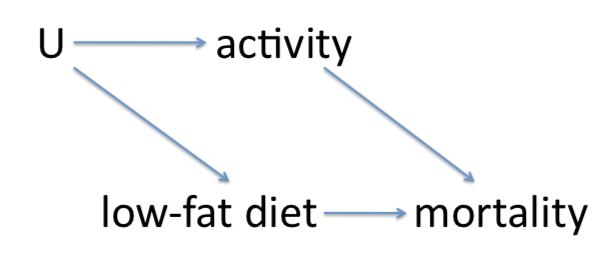
\includegraphics{data/dag.png}

\begin{enumerate}
\def\labelenumi{(\alph{enumi})}
\setcounter{enumi}{2}
\item
  For each of the four strata of physical activity, calculate a point
  estimate for the odds ratio comparing low-fat diet to other diets.
  \[\widehat{OR}_0  = \frac{17 \times 75}{75 \times 22} = 0.77\]
  \[\widehat{OR}_1  = \frac{28 \times 45}{40 \times 36} = 0.88\]
  \[\widehat{OR}_2  = \frac{10 \times 34}{14 \times 37} = 0.66\]
  \[\widehat{OR}_3  = \frac{4 \times 32}{7 \times 24} = 0.76\]
\item
  Based on your results in (c), does it seem plausible that the effect
  of low-fat diet on mortality (as measured on the odds ratio scale) is
  the same in all four groups of physical activity?
\end{enumerate}

Yes, the four separate odds ratio estimates are all fairly close
together.

\begin{enumerate}
\def\labelenumi{(\alph{enumi})}
\setcounter{enumi}{4}
\tightlist
\item
  Let's assume for the remainder of this question that the effect of
  low-fat diet on mortality is in fact the same at all four levels of
  physical activity. Carry out the Cochran-Mantel-Haenszel test to
  evaluate the null hypothesis that low-fat diet is not associated with
  mortality in any of the four strata of physical activity. What is the
  alternative hypothesis of this test? What is your conclusion?
\end{enumerate}

The alternative hypothesis is that \(OR_0 = OR_1 = OR_2 = OR_3 \neq 1\).
\[\chi^2_{CMH} = \frac{(59 - 64.663)^2}{23.694} = 1.353\]
\[p = 0.245 \text{ (from chi squared distribution)}\]

Based on the CMH test, we do not reject the null at the .05 level. In
other words, this test does not provide support for the conjecture that
low-fat diet is associated with mortality after controlling
(stratifying) on activity level (assuming no multiplicative
interaction).

\begin{enumerate}
\def\labelenumi{(\alph{enumi})}
\setcounter{enumi}{5}
\tightlist
\item
  Calculate an individual \(\chi^2\)-statistic for testing independence
  between low-fat diet and mortality in each stratum. Compare the sum of
  these four statistics against a \(\chi^2\) distribution with four
  degrees of freedom. What is the alternative hypothesis for the test
  that you just calculated a p-value for? Compare your p-value to the
  one you calculated in (e) and explain any difference you might see.
\end{enumerate}

The alternative hypothesis for this test is that at least one of the
stratum-specific ORs is not equal to 1 (i.e., the alternative is that
there is a relationship between low-fat diet and mortality in at least
one of the stratum, making no assumption regarding statistical
interactions). Notice the difference between this null hypothesis and
the one in (e), in particular that there is no assumption here of no
multiplicative interaction so that this alternative is broader. Here is
a table summarizing the information we need:

\begin{longtable}[]{@{}rr@{}}
\toprule
Activity.Level & Chi.Square\tabularnewline
\midrule
\endhead
0 & 0.51\tabularnewline
1 & 0.16\tabularnewline
2 & 0.78\tabularnewline
3 & 0.16\tabularnewline
\bottomrule
\end{longtable}

Lower power because alternative hypothesis is broader.

\begin{enumerate}
\def\labelenumi{(\alph{enumi})}
\setcounter{enumi}{6}
\tightlist
\item
  Calculate a Mantel-Haenszel point estimate for the summary odds ratio.
\end{enumerate}

Here is a table summarizing the information we need:

\begin{longtable}[]{@{}rrr@{}}
\toprule
Activity.Level & ad.n & bc.n\tabularnewline
\midrule
\endhead
0 & 6.746 & 8.730\tabularnewline
1 & 8.456 & 9.664\tabularnewline
2 & 3.579 & 5.453\tabularnewline
3 & 1.910 & 2.507\tabularnewline
\$\$\widehat{OR}\_\{M & H\} = \fr & ac\{20.691\}\{26.354\} =
0.79\$\$\tabularnewline
\bottomrule
\end{longtable}

\begin{enumerate}
\def\labelenumi{(\alph{enumi})}
\setcounter{enumi}{7}
\tightlist
\item
  Calculate a Woolf estimate and corresponding 95\% confidence interval
  for the summary odds ratio. \vspace{200pt}
\end{enumerate}

Here is a table summarizing the information we need:

\begin{longtable}[]{@{}rrr@{}}
\toprule
Activity.Level & log.or & bc.n\tabularnewline
\midrule
\endhead
0 & -0.251 & 7.801\tabularnewline
1 & -0.131 & 9.161\tabularnewline
2 & -0.406 & 4.548\tabularnewline
3 & -0.228 & 2.341\tabularnewline
\$\$\textbackslash{}log\{\textbackslash{}widehat\{O & R\}\_W\} = \ &
frac\{(-0.251) \times 7.801 + \ldots{} + (-0.228)
\times 2.341\}\{23.859\} = -0.232\$\$\tabularnewline
\$\$\widehat{OR}\_W & = \textbackslash{}exp\{(- & 0.232)\} =
0.793\$\$\tabularnewline
\$\$\widehat{var}\B & ig(\textbackslash{}log\{( & \widehat{OR}\_W)\}
\Big) = \frac{1}{23.859} = 0.0419\$\$\tabularnewline
\$\$\textbackslash{}text\{95\% CI fo & r log(OR) & \} = -0.232 \pm 1.96
\sqrt{0.0419} = (-0.633, 0.169)\$\$\tabularnewline
\$\$\textbackslash{}text\{95\% CI fo & r OR\} = ( & 0.53,
1.18)\$\$\tabularnewline
\bottomrule
\end{longtable}

\begin{enumerate}
\def\labelenumi{(\roman{enumi})}
\tightlist
\item
  Compare your two adjusted estimates in (g) and (h) to the crude
  estimate in (a). Is the relationship between low-fat diet and
  mortality confounded?
\end{enumerate}

Yes, since the adjusted estimated is substantially different from the
crude estimate, there is confounding (we know from the DAG above that
activity is neither a collider nor on the causal pathway so
non-collapsibility and confounding are equivalent here).

\begin{enumerate}
\def\labelenumi{(\alph{enumi})}
\setcounter{enumi}{9}
\tightlist
\item
  Check your calculations for (a), (c), (e), and (g) in R and show your
  output. You will need to use \texttt{epitab()} and
  \texttt{mantelhaen.test()}.
\end{enumerate}

\begin{Shaded}
\begin{Highlighting}[]
\CommentTok{# (a)}
\KeywordTok{epitab}\NormalTok{(}\KeywordTok{c}\NormalTok{(}\DecValTok{59}\NormalTok{, }\DecValTok{119}\NormalTok{, }\DecValTok{136}\NormalTok{, }\DecValTok{186}\NormalTok{))}
\end{Highlighting}
\end{Shaded}

\begin{verbatim}
## $tab
##           Outcome
## Predictor  Disease1        p0 Disease2        p1 oddsratio    lower
##   Exposed1       59 0.3025641      119 0.3901639 1.0000000       NA
##   Exposed2      136 0.6974359      186 0.6098361 0.6780771 0.462563
##           Outcome
## Predictor      upper    p.value
##   Exposed1        NA         NA
##   Exposed2 0.9940021 0.05535248
## 
## $measure
## [1] "wald"
## 
## $conf.level
## [1] 0.95
## 
## $pvalue
## [1] "fisher.exact"
\end{verbatim}

\begin{Shaded}
\begin{Highlighting}[]
\CommentTok{# (c)}
\KeywordTok{epitab}\NormalTok{(}\KeywordTok{c}\NormalTok{(}\DecValTok{17}\NormalTok{, }\DecValTok{22}\NormalTok{, }\DecValTok{75}\NormalTok{, }\DecValTok{75}\NormalTok{))}\OperatorTok{$}\NormalTok{tab}
\end{Highlighting}
\end{Shaded}

\begin{verbatim}
##           Outcome
## Predictor  Disease1        p0 Disease2        p1 oddsratio     lower
##   Exposed1       17 0.1847826       22 0.2268041 1.0000000        NA
##   Exposed2       75 0.8152174       75 0.7731959 0.7727273 0.3801964
##           Outcome
## Predictor     upper   p.value
##   Exposed1       NA        NA
##   Exposed2 1.570524 0.5899974
\end{verbatim}

\begin{Shaded}
\begin{Highlighting}[]
\KeywordTok{epitab}\NormalTok{(}\KeywordTok{c}\NormalTok{(}\DecValTok{28}\NormalTok{, }\DecValTok{36}\NormalTok{, }\DecValTok{40}\NormalTok{, }\DecValTok{45}\NormalTok{))}\OperatorTok{$}\NormalTok{tab}
\end{Highlighting}
\end{Shaded}

\begin{verbatim}
##           Outcome
## Predictor  Disease1        p0 Disease2        p1 oddsratio     lower
##   Exposed1       28 0.4117647       36 0.4444444     1.000        NA
##   Exposed2       40 0.5882353       45 0.5555556     0.875 0.4558074
##           Outcome
## Predictor     upper  p.value
##   Exposed1       NA       NA
##   Exposed2 1.679712 0.741056
\end{verbatim}

\begin{Shaded}
\begin{Highlighting}[]
\KeywordTok{epitab}\NormalTok{(}\KeywordTok{c}\NormalTok{(}\DecValTok{10}\NormalTok{, }\DecValTok{37}\NormalTok{, }\DecValTok{14}\NormalTok{, }\DecValTok{34}\NormalTok{))}\OperatorTok{$}\NormalTok{tab}
\end{Highlighting}
\end{Shaded}

\begin{verbatim}
##           Outcome
## Predictor  Disease1        p0 Disease2        p1 oddsratio     lower
##   Exposed1       10 0.4166667       37 0.5211268 1.0000000        NA
##   Exposed2       14 0.5833333       34 0.4788732 0.6563707 0.2575279
##           Outcome
## Predictor     upper   p.value
##   Exposed1       NA        NA
##   Exposed2 1.672916 0.4800262
\end{verbatim}

\begin{Shaded}
\begin{Highlighting}[]
\KeywordTok{epitab}\NormalTok{(}\KeywordTok{c}\NormalTok{(}\DecValTok{4}\NormalTok{, }\DecValTok{24}\NormalTok{, }\DecValTok{7}\NormalTok{, }\DecValTok{32}\NormalTok{))}\OperatorTok{$}\NormalTok{tab}
\end{Highlighting}
\end{Shaded}

\begin{verbatim}
## Warning in chisq.test(xx, correct = correction): Chi-squared approximation
## may be incorrect
\end{verbatim}

\begin{verbatim}
##           Outcome
## Predictor  Disease1        p0 Disease2        p1 oddsratio     lower
##   Exposed1        4 0.3636364       24 0.4285714 1.0000000        NA
##   Exposed2        7 0.6363636       32 0.5714286 0.7619048 0.1999751
##           Outcome
## Predictor     upper   p.value
##   Exposed1       NA        NA
##   Exposed2 2.902856 0.7504788
\end{verbatim}

\begin{Shaded}
\begin{Highlighting}[]
\CommentTok{# (e)}
\KeywordTok{mantelhaen.test}\NormalTok{(}
\KeywordTok{array}\NormalTok{(}\KeywordTok{c}\NormalTok{(}\DecValTok{17}\NormalTok{, }\DecValTok{22}\NormalTok{, }\DecValTok{75}\NormalTok{, }\DecValTok{75}\NormalTok{,}
  \DecValTok{28}\NormalTok{, }\DecValTok{36}\NormalTok{, }\DecValTok{40}\NormalTok{, }\DecValTok{45}\NormalTok{,}
  \DecValTok{10}\NormalTok{, }\DecValTok{37}\NormalTok{, }\DecValTok{14}\NormalTok{, }\DecValTok{34}\NormalTok{,}
  \DecValTok{4}\NormalTok{, }\DecValTok{24}\NormalTok{, }\DecValTok{7}\NormalTok{, }\DecValTok{32}\NormalTok{), }\DataTypeTok{dim =} \KeywordTok{c}\NormalTok{(}\DecValTok{2}\NormalTok{, }\DecValTok{2}\NormalTok{, }\DecValTok{4}\NormalTok{)), }
  \DataTypeTok{correct =} \OtherTok{FALSE}\NormalTok{)}
\end{Highlighting}
\end{Shaded}

\begin{verbatim}
## 
##  Mantel-Haenszel chi-squared test without continuity correction
## 
## data:  array(c(17, 22, 75, 75, 28, 36, 40, 45, 10, 37, 14, 34, 4, 24,     7, 32), dim = c(2, 2, 4))
## Mantel-Haenszel X-squared = 1.3534, df = 1, p-value = 0.2447
## alternative hypothesis: true common odds ratio is not equal to 1
## 95 percent confidence interval:
##  0.5228808 1.1789039
## sample estimates:
## common odds ratio 
##         0.7851281
\end{verbatim}

\begin{Shaded}
\begin{Highlighting}[]
\CommentTok{# (g)}
\KeywordTok{mantelhaen.test}\NormalTok{(}
\KeywordTok{array}\NormalTok{(}\KeywordTok{c}\NormalTok{(}\DecValTok{17}\NormalTok{, }\DecValTok{22}\NormalTok{, }\DecValTok{75}\NormalTok{, }\DecValTok{75}\NormalTok{,}
        \DecValTok{28}\NormalTok{, }\DecValTok{36}\NormalTok{, }\DecValTok{40}\NormalTok{, }\DecValTok{45}\NormalTok{,}
        \DecValTok{10}\NormalTok{, }\DecValTok{37}\NormalTok{, }\DecValTok{14}\NormalTok{, }\DecValTok{34}\NormalTok{,}
        \DecValTok{4}\NormalTok{, }\DecValTok{24}\NormalTok{, }\DecValTok{7}\NormalTok{, }\DecValTok{32}\NormalTok{), }\DataTypeTok{dim =} \KeywordTok{c}\NormalTok{(}\DecValTok{2}\NormalTok{, }\DecValTok{2}\NormalTok{, }\DecValTok{4}\NormalTok{)), }
        \DataTypeTok{correct =} \OtherTok{FALSE}\NormalTok{)}\OperatorTok{$}\NormalTok{conf.int}
\end{Highlighting}
\end{Shaded}

\begin{verbatim}
## [1] 0.5228808 1.1789039
## attr(,"conf.level")
## [1] 0.95
\end{verbatim}


\end{document}
